\documentclass[	
	12pt, % defining font size
	a4paper, % defining paper size
]{scrartcl}\usepackage[]{graphicx}\usepackage[]{color}
%% maxwidth is the original width if it is less than linewidth
%% otherwise use linewidth (to make sure the graphics do not exceed the margin)
\makeatletter
\def\maxwidth{ %
  \ifdim\Gin@nat@width>\linewidth
    \linewidth
  \else
    \Gin@nat@width
  \fi
}
\makeatother

\definecolor{fgcolor}{rgb}{0.345, 0.345, 0.345}
\newcommand{\hlnum}[1]{\textcolor[rgb]{0.686,0.059,0.569}{#1}}%
\newcommand{\hlstr}[1]{\textcolor[rgb]{0.192,0.494,0.8}{#1}}%
\newcommand{\hlcom}[1]{\textcolor[rgb]{0.678,0.584,0.686}{\textit{#1}}}%
\newcommand{\hlopt}[1]{\textcolor[rgb]{0,0,0}{#1}}%
\newcommand{\hlstd}[1]{\textcolor[rgb]{0.345,0.345,0.345}{#1}}%
\newcommand{\hlkwa}[1]{\textcolor[rgb]{0.161,0.373,0.58}{\textbf{#1}}}%
\newcommand{\hlkwb}[1]{\textcolor[rgb]{0.69,0.353,0.396}{#1}}%
\newcommand{\hlkwc}[1]{\textcolor[rgb]{0.333,0.667,0.333}{#1}}%
\newcommand{\hlkwd}[1]{\textcolor[rgb]{0.737,0.353,0.396}{\textbf{#1}}}%

\usepackage{framed}
\makeatletter
\newenvironment{kframe}{%
 \def\at@end@of@kframe{}%
 \ifinner\ifhmode%
  \def\at@end@of@kframe{\end{minipage}}%
  \begin{minipage}{\columnwidth}%
 \fi\fi%
 \def\FrameCommand##1{\hskip\@totalleftmargin \hskip-\fboxsep
 \colorbox{shadecolor}{##1}\hskip-\fboxsep
     % There is no \\@totalrightmargin, so:
     \hskip-\linewidth \hskip-\@totalleftmargin \hskip\columnwidth}%
 \MakeFramed {\advance\hsize-\width
   \@totalleftmargin\z@ \linewidth\hsize
   \@setminipage}}%
 {\par\unskip\endMakeFramed%
 \at@end@of@kframe}
\makeatother

\definecolor{shadecolor}{rgb}{.97, .97, .97}
\definecolor{messagecolor}{rgb}{0, 0, 0}
\definecolor{warningcolor}{rgb}{1, 0, 1}
\definecolor{errorcolor}{rgb}{1, 0, 0}
\newenvironment{knitrout}{}{} % an empty environment to be redefined in TeX

\usepackage{alltt}

%----------------------------------------------------------------------
% INCLUDE PACKAGES:

\usepackage{graphicx} % needed to able to include graphics
\usepackage{cmbright} % for a clone of Helvetica font
\usepackage[
    automark, % put sectionname into heading
    headsepline, % put a line under the heading  
]{scrpage2}
\usepackage{tikz}
\usepackage{booktabs} % needed for table
\usepackage{multirow} % used for tables
\usepackage{tabularx}
\usepackage[bf, nooneline, footnotesize]{caption} % define caption style
\usepackage{subfig}
\usepackage[paper=a4paper,top=20mm,bottom=30mm,left=30mm,right=20mm,footskip=10mm]{geometry} % defining text boarders to define geometry of the article according to dvs-standards
\usepackage{import} % to be able to use the \import command (use in combination of svg graphics produced mainly with inkscape)
\usepackage{todonotes}
\usepackage{url} % url package needed to define url look at references
\usepackage[colorlinks=true,citecolor=blue,urlcolor=blue, linkcolor=black]{hyperref} % create the links in the document
\usepackage{apacite} % citation package

%----------------------------------------------------------------------
% DOCUMENT DEFINITIONS:

\pagestyle{scrheadings} % create heading
\renewcommand*\familydefault{\sfdefault} %for a clone of Helvetica font
\newcommand*\mytitle{The effect of diversity on team performance and team satisfaction in German amateur football clubs} % define title
\ihead{\mytitle} % show title in header and align it to the left
\chead{} % no title in centered part of header
\linespread{1.5} % define linespread
\title{\mytitle}
\subtitle{Final paper}
\author{
        N. McCown, M. Metz, T. Prenzel, C. Xi\\
        Institute of Sport Economics and Sport Management\\
        German Sport University Cologne\\
        }
\date{\today}

%---------------------------------------------------------------------
% BEGINNING OF DOCUMENT:
\IfFileExists{upquote.sty}{\usepackage{upquote}}{}
\begin{document}
\pagenumbering{Roman}

%---------------------------------------------------------------------
% INPUT TITLEPAGE:

\newgeometry{margin=20mm} % geometry settings for titlepage
\begin{titlepage}
\pagenumbering{Roman} % start with roman page numbers
\maketitle
     \vspace{2cm} % some vertical space       
\begin{center}

\includegraphics[scale=0.9]{logo_dshs_01.jpg}
\end{center}
\vspace{2cm} % some vertical space
\begin{center}
\begin{tabular}{rl}
Matr.Nr.: &480619; 481269; 481612; 480448 \\ 
E-Mail: &\href{mailto:nmccown@gmail.com}{nmccown@gmail.com}; \href{mailto:metz.magnus@gmail.com}{metz.magnus@gmail.com};\\ &\href{mailto:tobias.prenzel@gmail.com}{tobias.prenzel@gmail.com};
 \href{mailto:xichidio@live.cn}{xichidio@live.cn} \\ 
Course: & Managing social problems of sport management \\
Lecturer: & Prof. Dr. Ilse Hartmann-Tews\\
Term: & Summer 2013
\end{tabular} 
\end{center}
\thispagestyle{empty} % no pagenumber on titlepage
\end{titlepage}


%---------------------------------------------------------------------
\restoregeometry % go back to original geometry settings, defined in the preambel
\reversemarginpar % to have the todonotes on the left margin
\newpage % guess what? New page begins here
\headsep15mm % distance of text body to header
\setcounter{page}{2} % start with page number II
\tableofcontents % Insert Table of Contents
\newpage % Yes right, new page
%\listoffigures
\newpage
\pagenumbering{arabic} % start with arabic page numbers instead of Roman page numbers
\setcounter{page}{1} % start with arabic pagenumber 1 
\urlstyle{same} % same font for the url's in the references as the normal text








%---------------------------------------------------------------------
% INPUT CONTENT:
\section{Introduction}
With the introduction of the "Charta der Vielfalt" in 2006 by German entrepreneurs, aiming at the support and appreciation of all employees, diversity got its own manifest in German (economic) society \cite{Vielfalt2006}. At its core level the diversity of all employees should become a part of the personal strategy and the organizational development of an enterprise. In this study the discussion about diversity in Germany is transferred to sport, especially to football representing one of the most favourite German leisure activities and the most represented sport in migrational sport clubs \cite{Breuer2010}. The purpose of this paper is to provide a descriptive view on diversity in football clubs and further analyse the impact, diversity may have on both, team performance and overall team satisfaction. 
In addition practical implications for club managers as well as scientific foundation for political sport initiatives, on how to best deal with potentially increased diversity in sport clubs is tried to derive. As diversity issues in sport were mostly addressed on an organizational level \cite{Knoppers2008, Cunningham2004, Cunningham2007a, Cunningham2007b}, this study represents an early attempt on diversity in team sports from a sport management perspective, so far only investigated by a few authors from the anglo-saxon area \cite{Timmerman2000, Waltemyer2006}.

\section{Literature review}
\label{sec:literature}

\subsection{State of the art literature on diversity}

In scientific literature the term diversity is described in a multitude of ways. A more generic explanation by \citeA{Cox1997} argues that diversity is "a mix of people in one social system who have distinctly different socially relevant group affiliations". A more managerial approach by \citeA[p.~802]{Jackson2003} describes diversity as a "distribution of personal attributes among interdependent members of a work unit". Within the context of management it is important to mention that proactive dealing with diversity follows the purpose of creating a climate in which potential advantages of the diverse group can be utilized and maximized, while at the same time potential disadvantages are minimized to foster a group's success \cite{Cox1997}. \citeA{Cunningham2006} provide a comprehensive overview in their introductory article in the special issue of the Journal of Sport Management about "Diversity issues in sport and leisure". According to them, diversity is measured on two different levels, the surface level and the deep level of diversity \cite{Cunningham2006}. The surface level considers socio-economical and demographic indicators like gender, age, race, income and other more visible indicators \cite{Fink2001, Siciliano1996}, while the deep level considers less visible factors regarding psychology and personality, like values, attitudes and beliefs.
Furthermore the research around diversity can be devided into three fields, naming categorical diversity, compositional diversity, and relational demography \cite{Cunningham2006, Tsui1999}.
In general diversity is analysed in the context of Management, Sociology and Psychology. This paper will focus mainly to attempt on an interdisciplinary approach from both, a sociological and managerial perspective. In order to assure the feasibility of the research project, mainly the surface level of diversity is going to be observed.

\subsection{Diversity in team sports}
Historically sport clubs were founded on the basis of identical ideas. Therefore club members would usually share the same cultural background, religion, sex, gender and form a club identity based on membership, participation and performance, which increased diversity in between the clubs further \cite{Anthonissen2001, Day1981}.

More recently diversity within sport clubs gained more academic attention, e.g. \citeA{Timmerman2000} found that age and racial diversity have a negative association with basketball team performance, however this relationship has not been found in the baseball sport. Thus, \citeA{Timmerman2000} argues that the relationship between diversity and team performance is inconsistent and mainly depends upon the interaction pattern in different sports. In addition \citeA{Waltemyer2006} found that ethnic diversity was significant and negatively related to team assists in the American National Hockey League (NHL).
The little existing knowledge on relationship between diversity and sport team performance tends to focus on the age diversity and racial diversity \cite{Pelled1999, Jehn1999, Waltemyer2006, Timmerman2000}. Moreover, only studies dealing with professional team sports were found with no regard to football. In order to fill this gap, and concentrating on amateur football, following two hypotheses are derived:

$ H_{1}: $ Higher diversity level in a team will positively affect team performance.

$ H_{2}: $ Higher diversity level will negatively affect team atmosphere satisfaction.


\section{Method}
\label{sec:method}
\subsection{Data collection}
The data collection was conducted stepwise. As a first step the target group of male amateur football players was identified. Primarily male participants were targeted, as it was assumed that interaction of team mates could differ across genders. Secondly, non-probability convenience sampling, more precisely snowball sampling, was used to get access to potential respondents. Study colleagues from our cohort, playing football by themselves, were asked to gather potential contact details of coaches, club officials and players from teams performing in German amateur leagues (4th division and lower). As far as practicable football clubs were visited in person by the authors during home games in order to increase survey participation through personal interaction. Third, the link to the on-line survey was distributed via the collected e-mail addresses and social media contacts, with the specific encouragement to distribute the link further to other team members and emphasizing the importance that as many team members as possible should participate in the survey. After two weeks of collection a reminder was sent to all contacts in order to further increase the participation rate. The questionnaire was created with the unipark software supplied by the German Sport University. The survey consisted of 14-15 questions on ten pages, using a progress bar to encourage the respondents' compliance. Finally, 148 people followed the link to our survey, of which 109 took part. After data cleansing the net sample size accounts for \textit{n}=71. 

\subsection{Measures} 
For the purpose of measuring team diversity, the respondents were asked to answer questions regarding their migrational background, religion, income, education, sexual orientation and age. Team atmosphere was measured using the Team Satisfaction Index Questionnaire \cite{Basadur2001}, where team members rate their satisfaction with their team experience on a one to ten scale for (1) how well they worked 
together; (2) how much fun they had; (3) how much desire they had to work with their team 
again; and (4) how good they felt about the quality of the output. Furthermore team success was measured through four specific questions asking for the league in which the respondents' team played, the current position in the league, games played during the season and games won during the season.

\subsection{Data analysis}
As a first step the overall sample was divided into eleven subsamples, each subsample representing one team. Next, some variables were recoded, indicating team atmosphere and team success. The variable team atmosphere was computed using the arithmetic mean of its indicators. A league index was calculated ranging from 0-1, where 1 indicated the highest league and 0 the lowest league possible. A further winning index consisting of the ratio between games played and games won gives information about the winning rate of a team. Finally team success was measured using the both indices mentioned above and calculating their arithmetic mean resulting in a value between 0 and 1, where 0 indicates the lowest team success and 1 the highest team success possible. For the purpose of quantifying Diversity within football teams, Blau's index was used for each category \cite{Blau1977}. According to Blau's index "Diversity = $ 1 - \sum p_i^{2} $ where \textit{p} is the proportion of group members in a racial category and \textit{i} is the number of different categories in a team" \cite[p.~599]{Timmerman2000}. High scores indicate greater diversity as lower scores. Age diversity is measured by the coefficient of variation (team\textit{SD}/team\textit{M}).




\section{Results}
\label{sec:results}

\begin{knitrout}\footnotesize
\definecolor{shadecolor}{rgb}{0.969, 0.969, 0.969}\color{fgcolor}\begin{figure}[]


{\centering 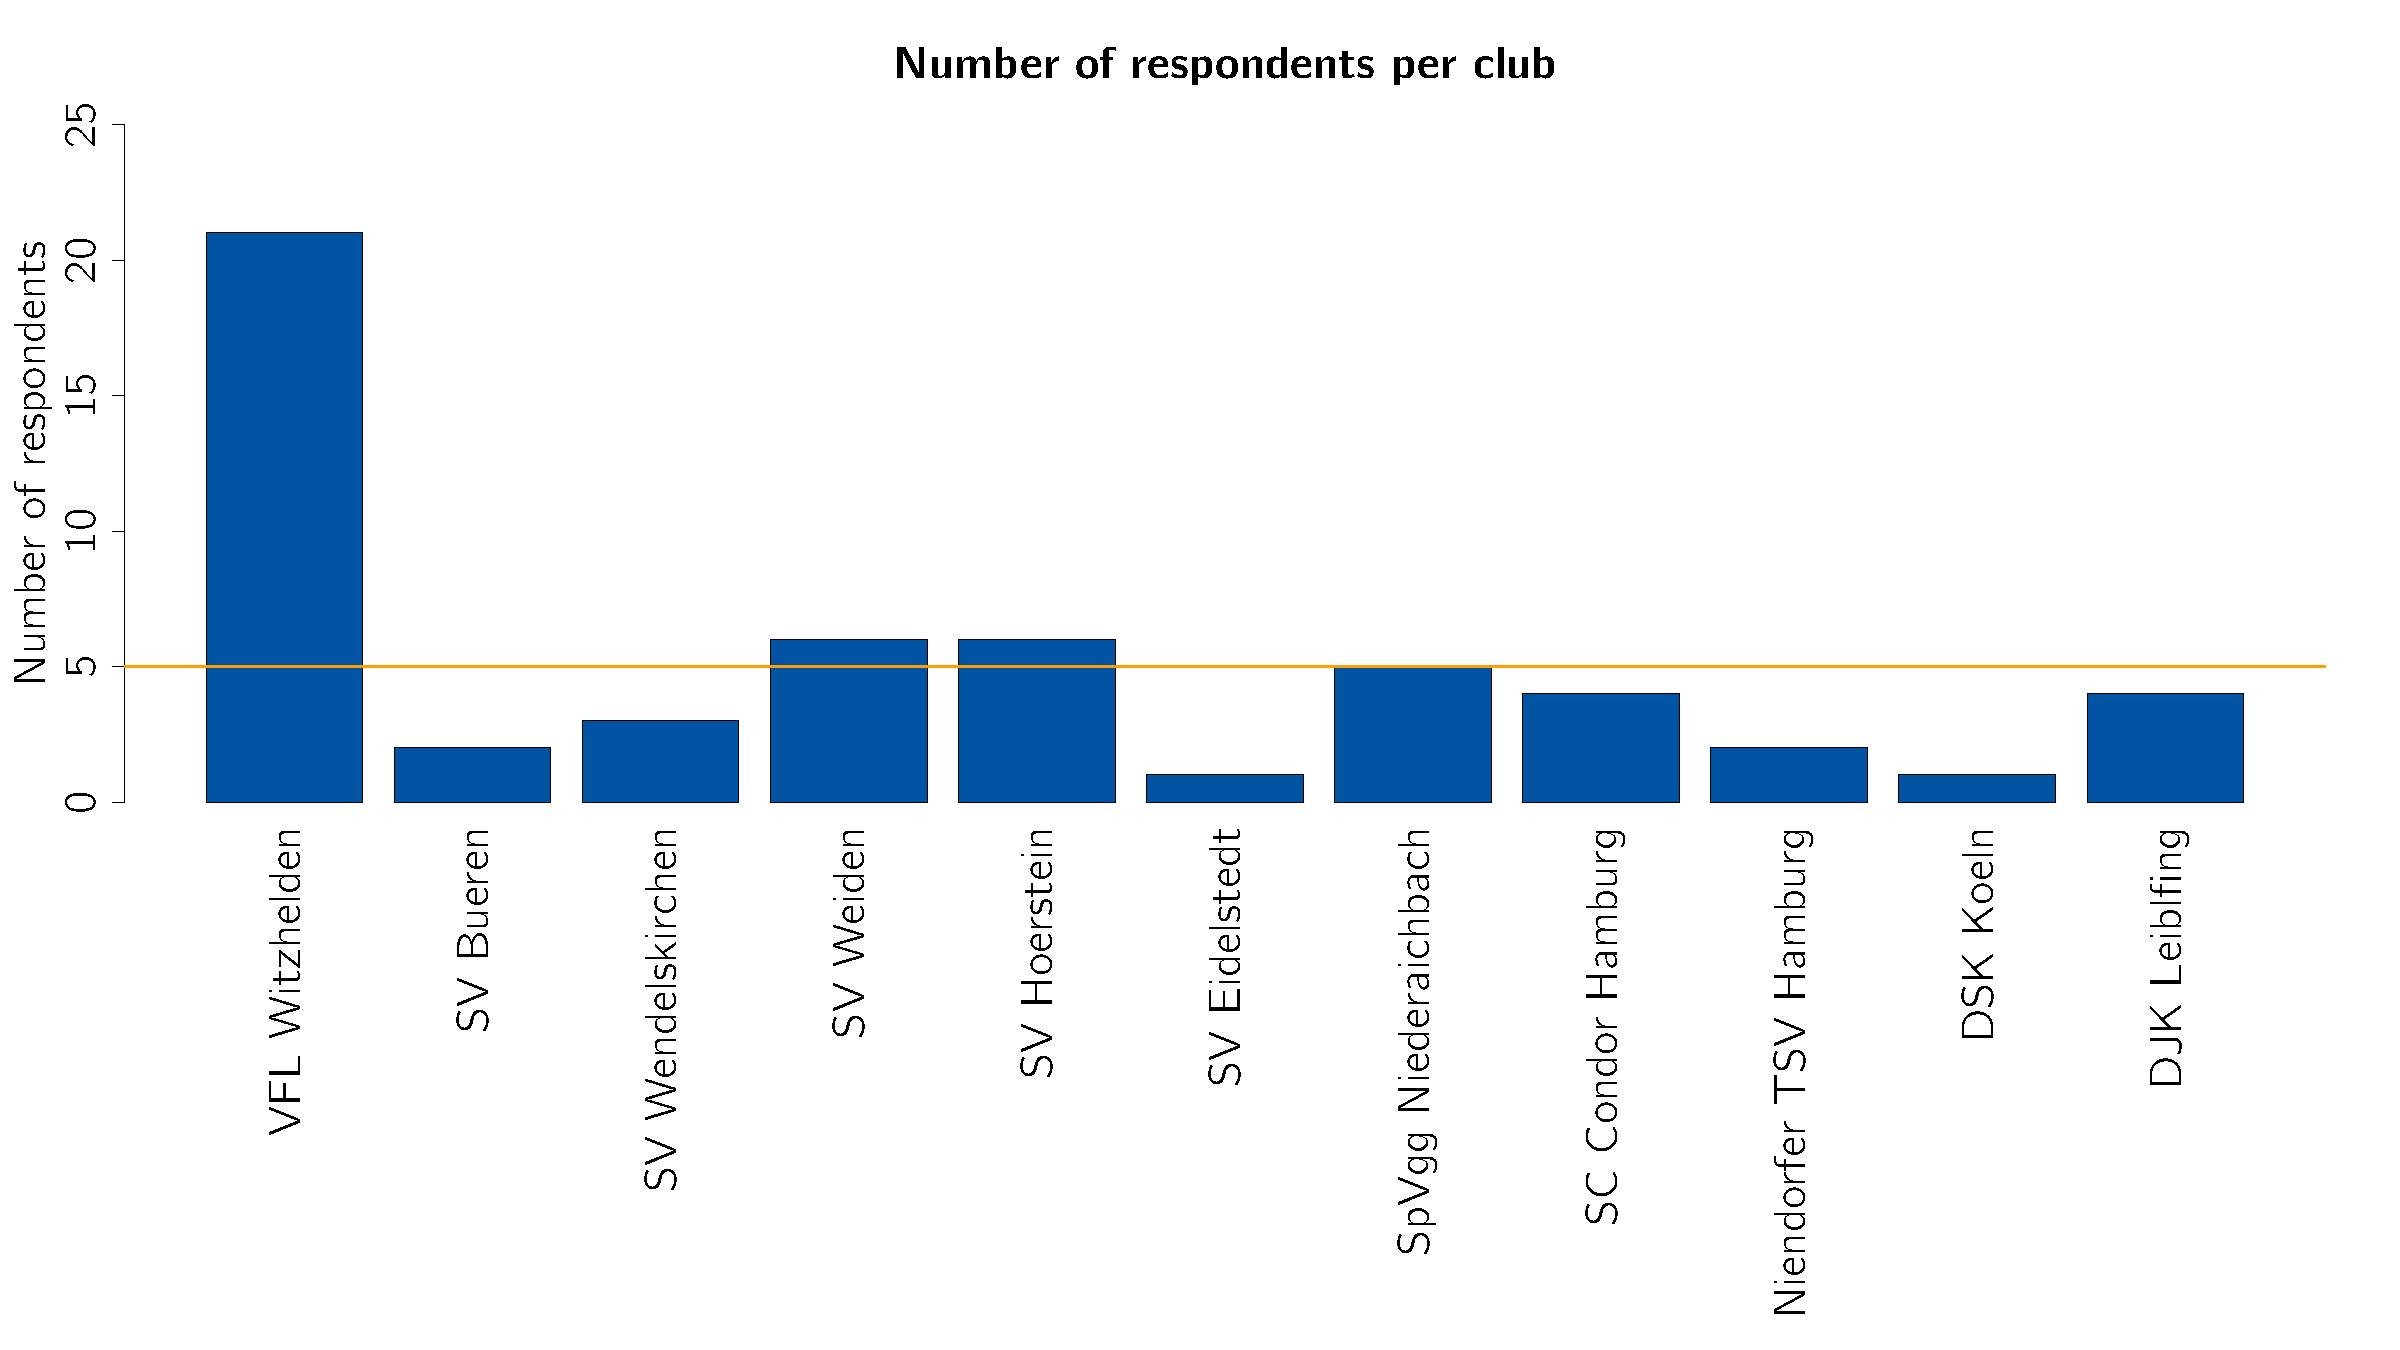
\includegraphics[width=1\linewidth]{figure/beamer-clubname} 

}

\caption[Number of respondents per club]{Number of respondents per club\label{fig:clubname}}
\end{figure}


\end{knitrout}


\begin{knitrout}\footnotesize
\definecolor{shadecolor}{rgb}{0.969, 0.969, 0.969}\color{fgcolor}\begin{figure}[]


{\centering 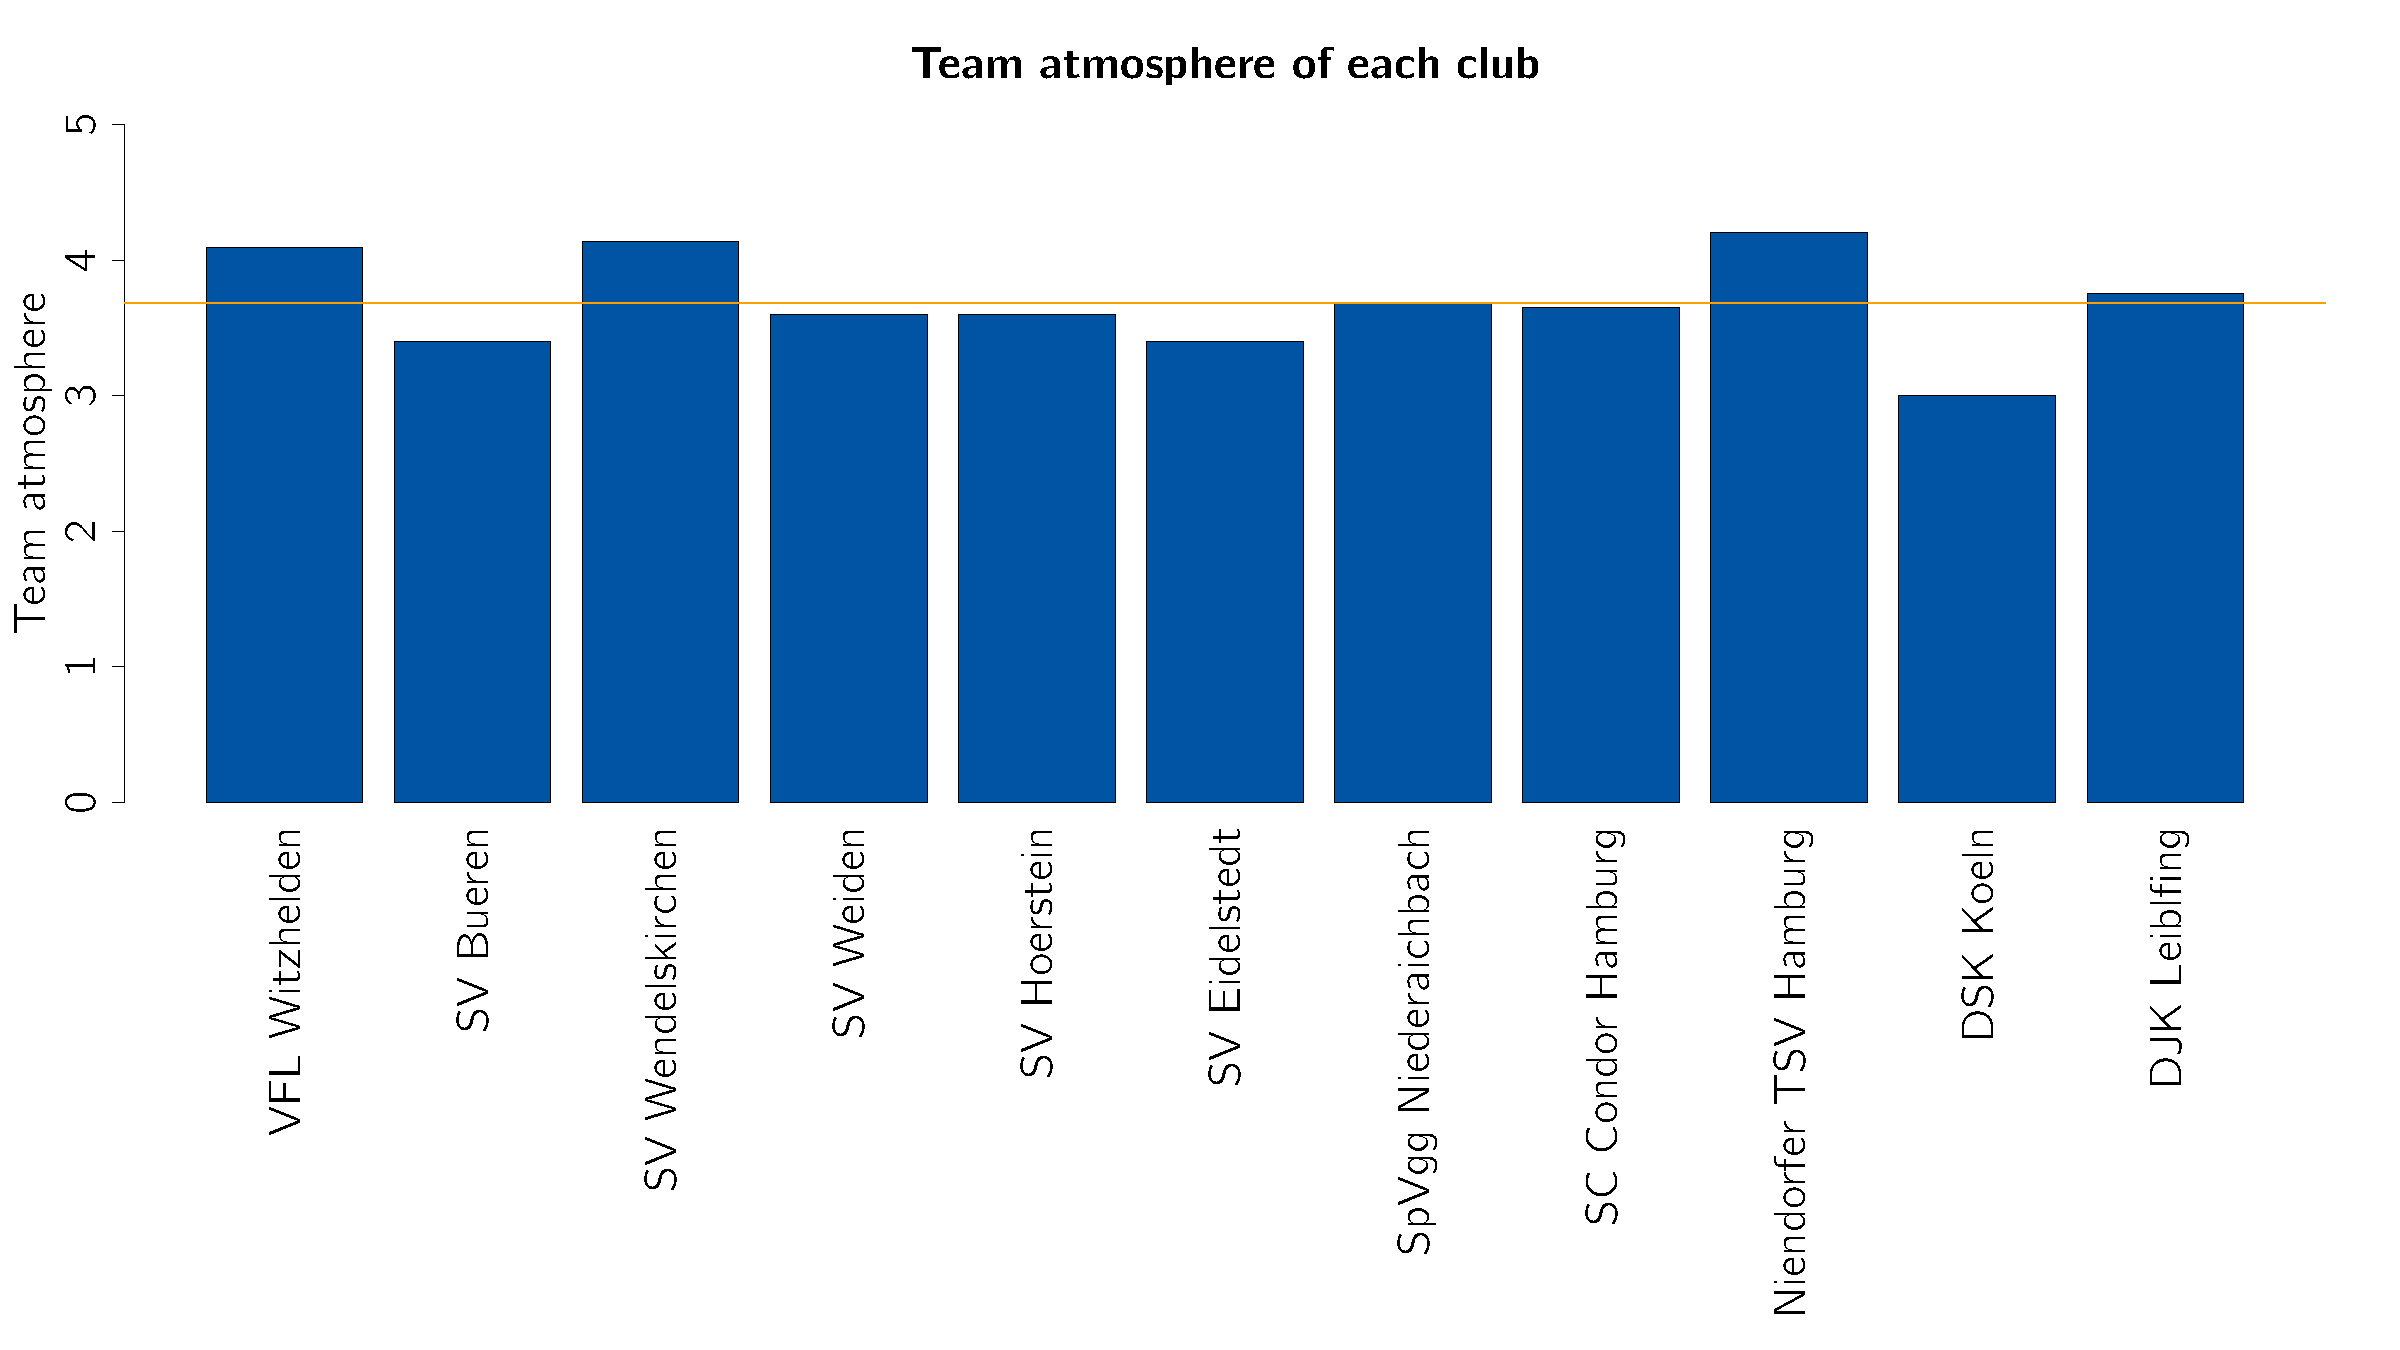
\includegraphics[width=1\linewidth]{figure/beamer-atmosphere} 

}

\caption[Team atmosphere of each club]{Team atmosphere of each club\label{fig:atmosphere}}
\end{figure}


\end{knitrout}


\begin{knitrout}\footnotesize
\definecolor{shadecolor}{rgb}{0.969, 0.969, 0.969}\color{fgcolor}\begin{figure}[]


{\centering 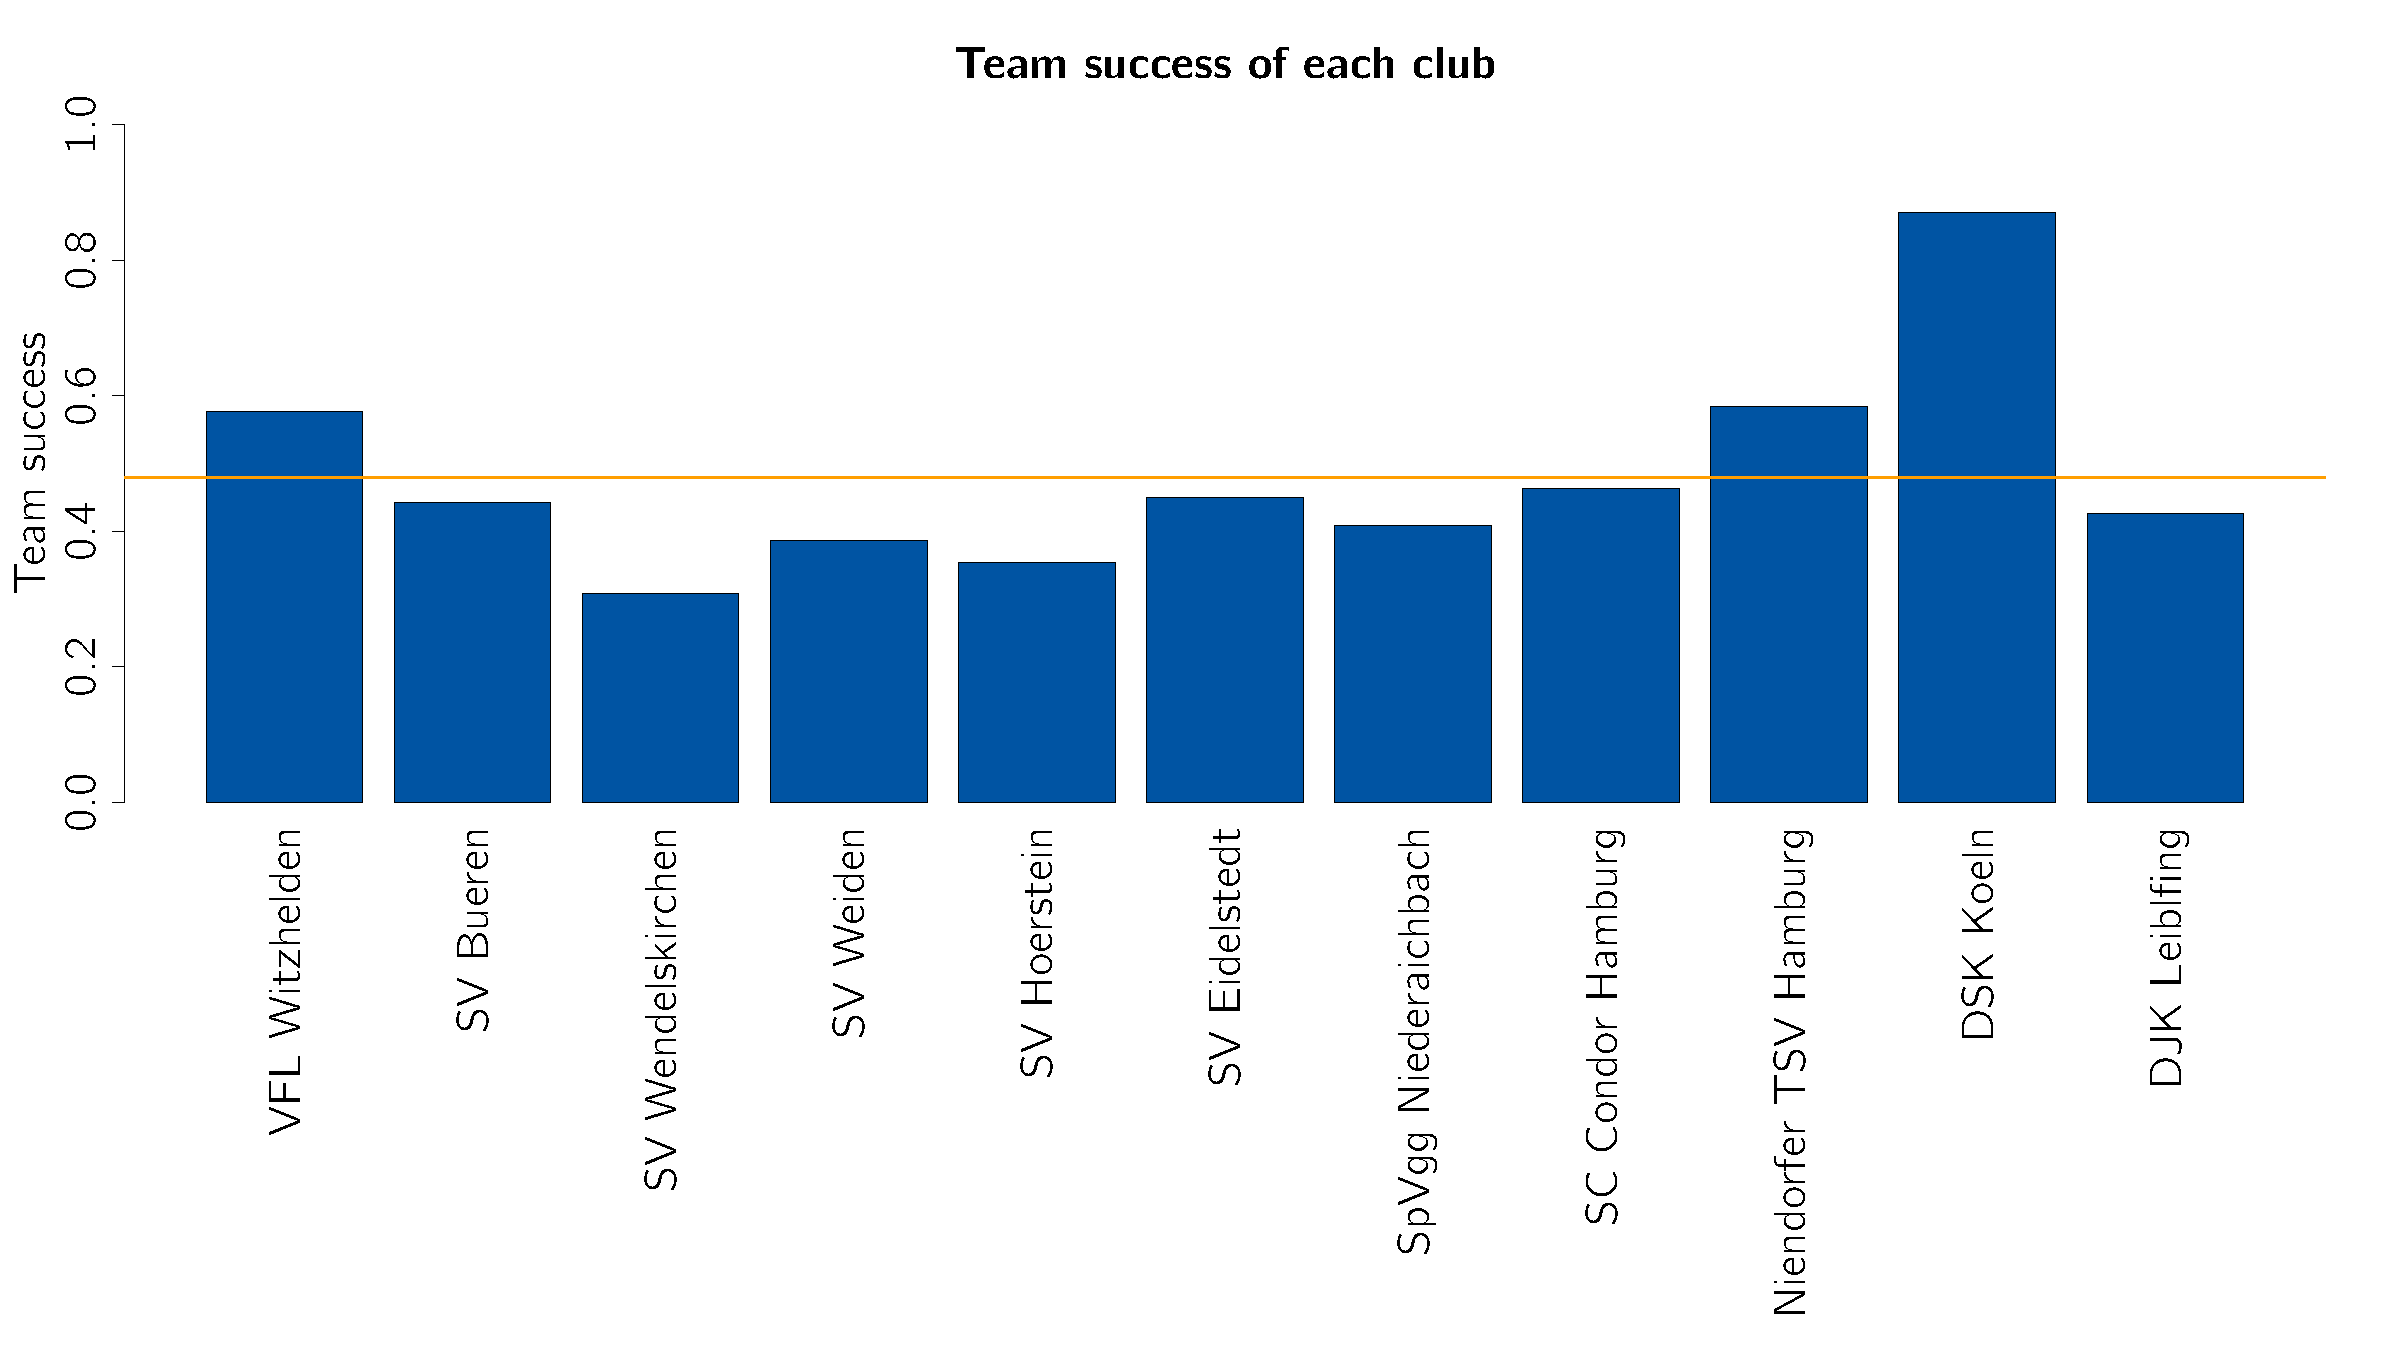
\includegraphics[width=1\linewidth]{figure/beamer-teamsuccess} 

}

\caption[Team success index of each club]{Team success index of each club\label{fig:teamsuccess}}
\end{figure}


\end{knitrout}


This section shows the results of our analysis. All values were computed for each club and graphically presented. Figure \ref{fig:clubname} shows representation of respondents in each club. The only club with a reasonable representation is VFL Witzhelden with 21 respondents. The participation of all other clubs has been significantly lower. The mean value for all clubs is 5 respondents. Figure \ref{fig:atmosphere} indicates the team atmosphere of each club. A quite equal distribution of team atmosphere among the clubs can be observed, with a mean value of 3.68. Figure \ref{fig:teamsuccess} shows the team success of each club. DSK Koeln seems to be the most successful club during the season 2012/2013, keeping in mind that the answer came from only one respondent. The mean value of team success for all clubs is 0.48. Table \ref{tab:indices} provides an overview of the diversity indices computed according to \citeA{Blau1977}. For a better overview all coefficients of table \ref{tab:indices} are also graphically presented in figure \ref{fig:indices}.

\begin{table}[htb]
\caption{Diversity indices of each club}
\centering
\begin{tabularx}{\textwidth}{lXXXXXX}
\toprule
  & Sex. orient. & Education & Income & Religion & Race & Age \\ 
\midrule
VFL Witzhelden & 0.00 & 0.76 &0.75 &0.62 &0.25&0.17 \\
SV Bueren & 0.00 & 0.50 & 0.00 & 0.00 & 0.50&0.33\\
SV Wendelskirchen & 0.00 & 0.44 & 0.44 & 0.00 & 0.00&0.07 \\
SV Weiden & 0.00 & 0.67 & 0.67 & 0.50 & 0.28 &0.34\\
SV Hoerstein & 0.28 & 0.61 & 0.78 & 0.67& 0.28&0.14 \\
SV Eidelstedt & 0.00 & 0.00 &0.00 &0.00 &0.00  &0.00\\
SpVgg Niederaichbach & 0.00 & 0.64 &0.50 &0.32 &0.32&0.12 \\
SC Condor Hamburg & 0.00 & 0.63 & 0.63& 0.44 & 0.00&0.08\\
Niendorfer TSV Hamburg & 0.00 & 0.50 & 0.50& 0.00&0.00&0.12 \\
DSK Koeln & 0.00 & 0.00 & 0.00 & 0.00 & 0.00  &0.00\\ 
DJK Leiblfing & 0.00 & 0.63 & 0.67 & 0.44 & 0.00&0.30 \\ 
\bottomrule
\end{tabularx} 
\begin{flushleft}
a. Age diversity was measured by the coefficient of variation (teamSD/teamM).\\
b. Racial diversity was measured with the index of \citeA{Blau1977}: $ 1 - \sum p_i^{2} $. \\
High scores indicate greater diversity.
\end{flushleft}
\label{tab:indices}
\end{table}



\begin{knitrout}\footnotesize
\definecolor{shadecolor}{rgb}{0.969, 0.969, 0.969}\color{fgcolor}\begin{figure}[]


{\centering 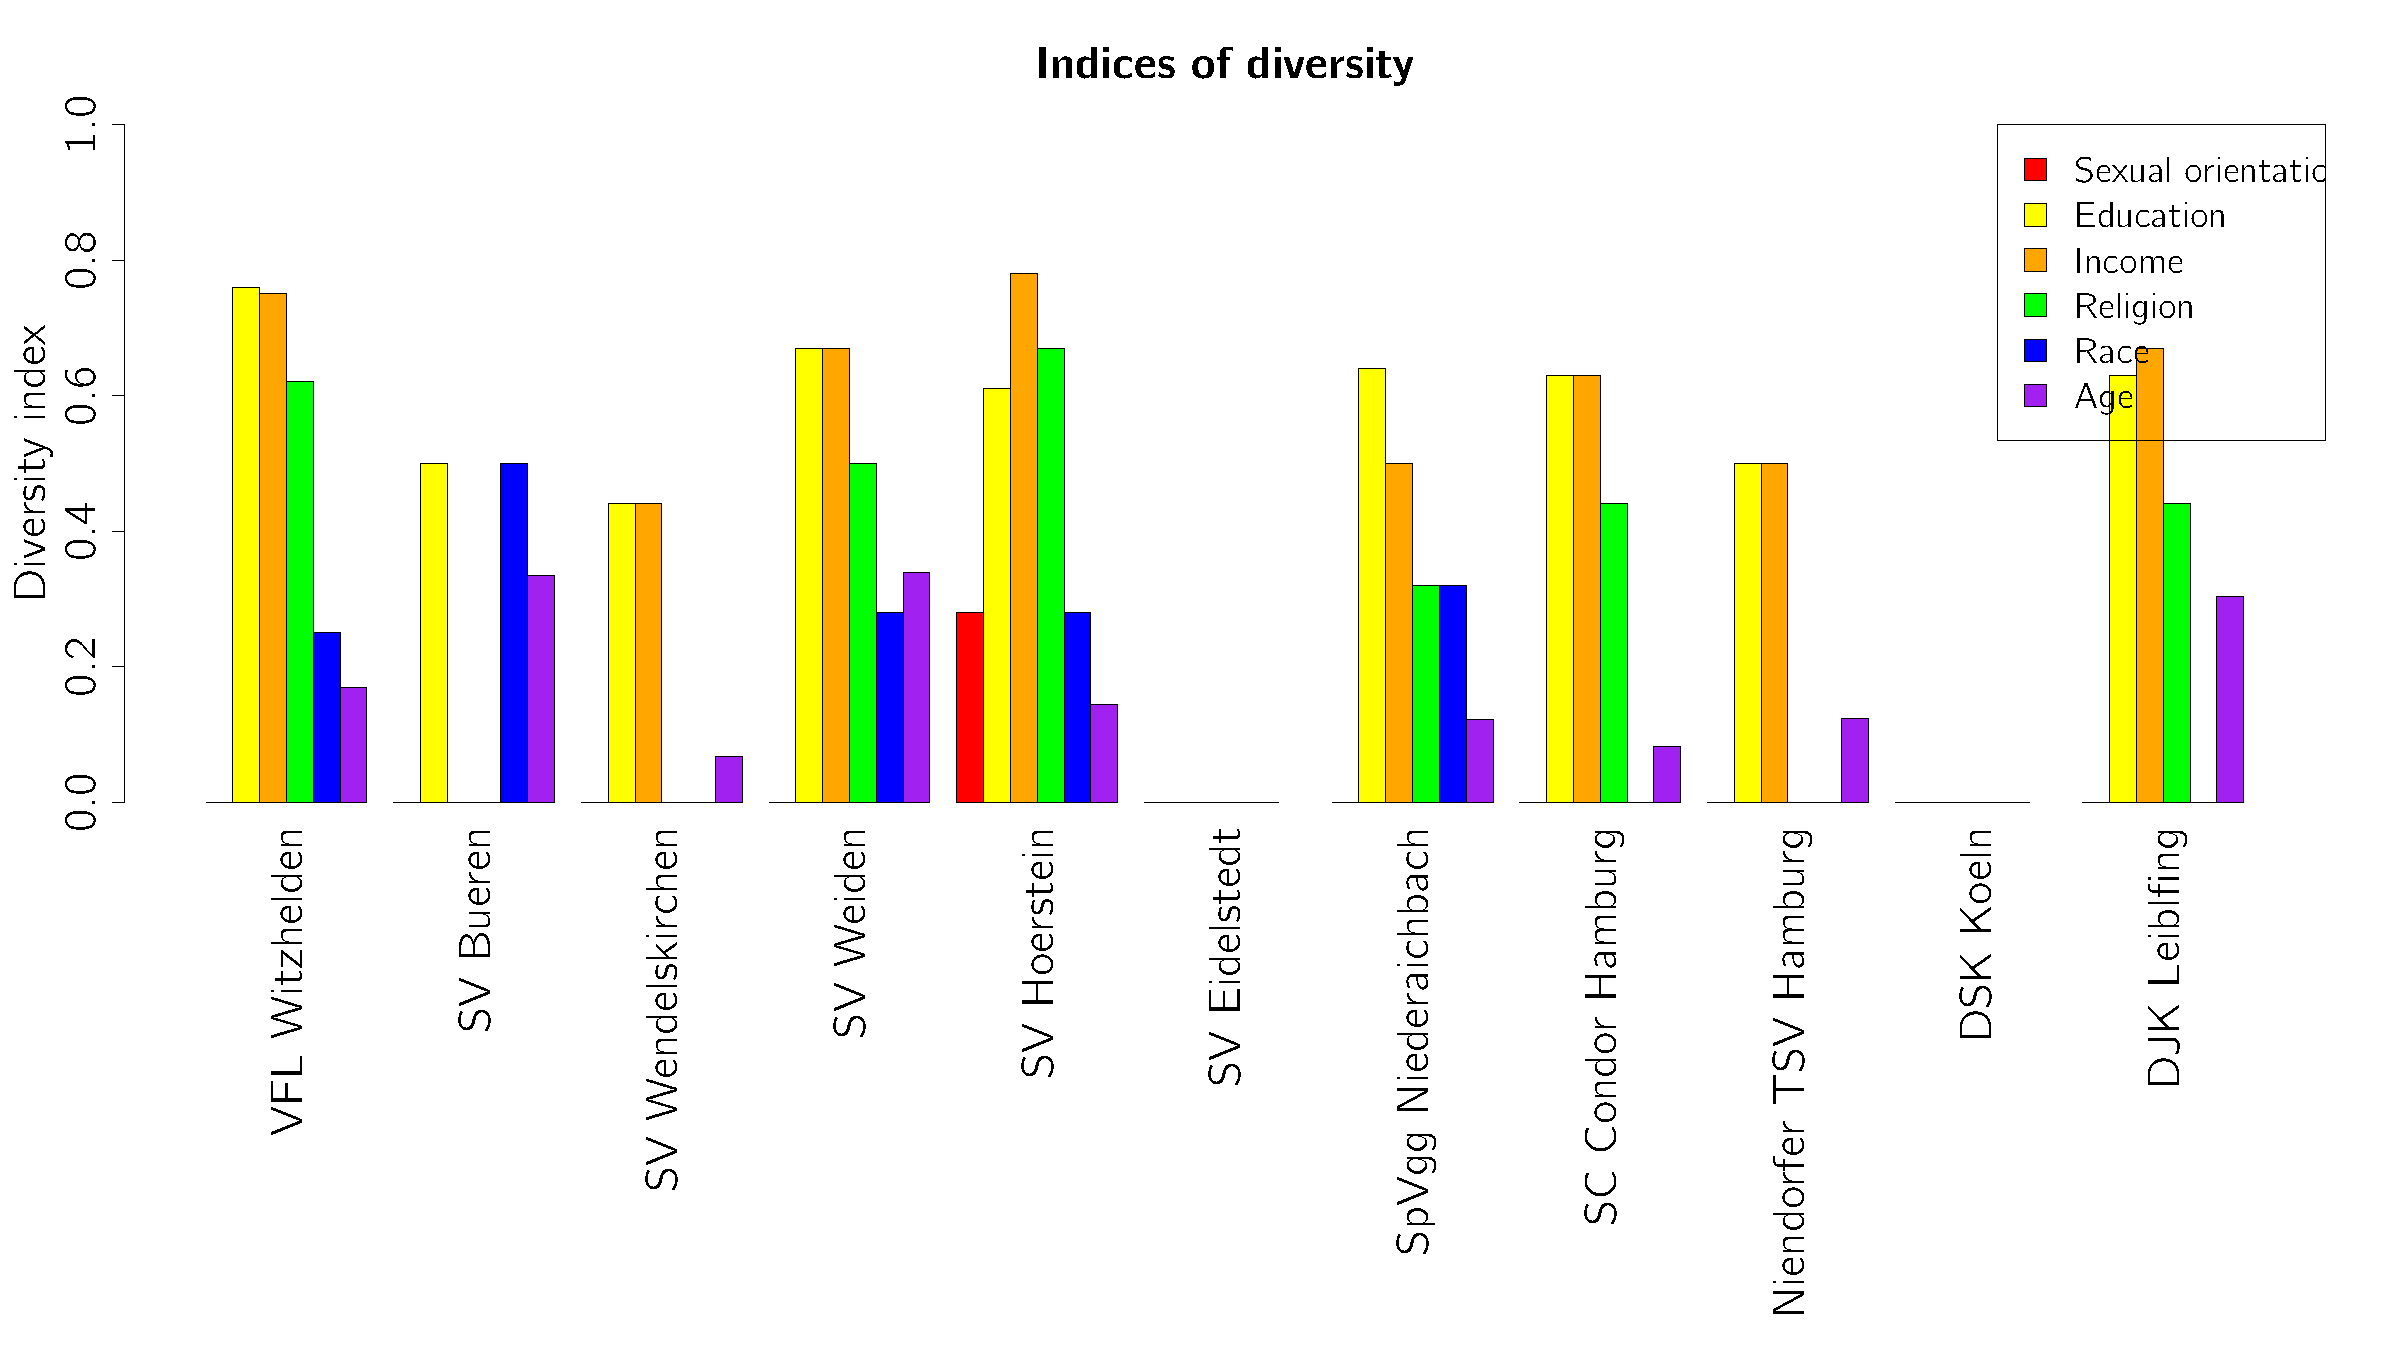
\includegraphics[width=1\linewidth]{figure/beamer-indices} 

}

\caption[Graphical representation of the diversity indices from table 1]{Graphical representation of the diversity indices from table 1\label{fig:indices}}
\end{figure}


\end{knitrout}



\clearpage

\section{Discussion}
\label{sec:discussion}
Considering the limitation of a low response rate the initial purpose of the study to compare diversity and its relationship with team atmosphere and success between different football clubs was deferred, due to limitations in sample size. This paper now concentrates on a simple descriptive observation and interpretation of the data.
The indices for diversity according to \citeA{Blau1977} indicate that in our subsamples diversity in race and especially sexual orientation is rather low, while diversity regarding income and education is considerably high within the clubs. Further the diversity with regards to the religion varies strongly in between the clubs. The observations can be interpreted as proof for the author’s assumption that sport clubs are not based on identical ideas anymore as they were historically, as described by \citeA{Anthonissen2001}. Neither do all club members share the same cultural background, nor religion or economical background. The open club system and globalisation in general seem to have reshuffled sport club memberships, which indeed resulted in the arrival of societal diversity into the football clubs. The lack of diversity with regards to race and sexual orientation within the samples at hand may be a simple representation of the societal diversity within the mostly rural areas, from which the samples were collated. But it might as well be due to the low level of acceptance of non-heterosexual relationships within those areas or in football in general and limited tolerance of foreigners, but these are assumptions, which need further sociological investigation. 
The diversity with regards to age of the players is rather low, which may be due to the nature of the sport, forcing older players to stop playing due to comparatively limited performance reasons. Another reason for the low diversity in age might as well be the non-random convenience sampling technique used by the authors that resulted in the recruitment of participants mainly between the age of 20 and 30.
As mentioned above, the data collected does not allow comparative interpretations on the influence of diversity within clubs on club´s success or atmosphere. Therefore the hypotheses $H_{1}$ and $H_{2}$ can neither be confirmed, nor rejected by our research. 
Simply observing the data on team success and atmosphere within the clubs, one is not able to conclude a relationship between diversity and success or atmosphere. Surprisingly, even between success and atmosphere within a club no relationship seems obvious, as some clubs with high indices for success show lower levels in atmosphere and vice-versa. This may be due to the low and unsatisfactory subsample size, or a result of the indices used to measure success and atmosphere. While the measures for atmosphere and success were derived from previous literature \cite{Basadur2001, Timmerman2000}, their utility in the research project at hand needs yet to be confirmed.


\section{Conclusion}
\label{sec:conclusion}
The findings from this research indicate that similar to the societal development towards more diversified communities with regards to cultural background, economical status, education and religion, the football clubs in Germany of which data has been collected here, show a considerably high diversity. Mainly with regards to education and income players of one club can be highly diversified, which is typical for the sport football that has rather low entry costs and is considered to be sport of the masses in Germany \cite{Breuer2010}. Unfortunately conclusions on the influence of diversity on variables like a club´s performance or the atmosphere within a club could not be made, due to limited subsample sizes.
\subsection{Practical implications}
As one of the pioneering research projects, attempting to apply diversity theory to the field of team sport, it has become clear that sport managers in football need to be aware and sensitive to the diversity within a club. High heterogeneity in income as well as education or religious affiliations can be the cause of issues within a club and need attention to facilitate maximum success. Further the satisfaction of individuals within a football club may highly depend on a manager´s ability to deal with the above-mentioned diversity in the right way.
\subsection{Limitations and future avenues}
While the research at hand needs to be seen as a first pioneer attempt, it is important to note that interpretation of results is limited. First, the collection of data can be improved by collating complete data from ideally all players of the respective teams. Focussing on one or two comparable leagues could further increase the quality of the results. Collaboration with national football associations e.g. the German Football League (DFL) might be of considerable advantage. Secondly, the survey can be improved, especially around areas that are perceived as sensitive by the participants, e.g. questions regarding sexual orientation. Here the usage of two techniques could be helpful to get more realistic data, the randomized response technique (RRT) and the unmatched count technique (UCT). Once better data has been collected, the avenues with regards to data analysis proposed in this paper, may lead to interesting revelations on the influence of different diversity aspects on the success of, and atmosphere in football clubs.

%---------------------------------------------------------------------
% BIBLIOGRAPHY:
\bibliographystyle{apacite}
\renewcommand{\bibliographytypesize}{\small} % set font size for bibliography
\interlinepenalty 10000 % no pagebreaks within citations
\bibliography{library} % defines the *.bib-file where your references are in. File needs to have the ending *.bib

\end{document}
